
\documentclass[10pt,twocolumn]{article}

% --------------------------------------------------
% Packages and formatting
% --------------------------------------------------

\usepackage[T1]{fontenc}
\usepackage[utf8]{inputenc}
\usepackage[margin=0.72in]{geometry}
\usepackage{times}
\usepackage{microtype}
\usepackage{booktabs}
\usepackage{graphicx}
\usepackage{amsmath}
\usepackage[numbers,sort&compress]{natbib}
\usepackage[hidelinks]{hyperref}
\usepackage{xcolor}
\usepackage{capt-of}
\usepackage{placeins}
\usepackage{balance}
\usepackage{url}

\setlength{\columnsep}{0.28in}
\setlength{\abovecaptionskip}{6pt}
\setlength{\belowcaptionskip}{2pt}

\renewcommand{\bibsection}{\section*{References}}
\bibliographystyle{plainnat}

% --------------------------------------------------
% Author information
% Named mentor-review / portfolio version
% --------------------------------------------------

\title{
A Shared Byte-Level BPE Vocabulary Uses More Held-Out
Tokens than Dedicated Vocabularies:
An English--Hindi--Nepali Study
}

\author{
Write authors name here
}

\date{}

% --------------------------------------------------

\begin{document}

\maketitle

% --------------------------------------------------
% Abstract
% --------------------------------------------------

\begin{abstract}

We investigate the held-out tokenization efficiency of shared
and language-specific byte-level byte-pair encoding (BPE)
vocabularies for English, Hindi, and Nepali.

Using a deterministic byte-level BPE implementation, we
compare dedicated and fully shared vocabularies under two
training-data regimes. At a requested vocabulary size of
1,024, three resampled training selections of approximately
300,000 UTF-8 bytes per language produce mean shared-vocabulary
token-count penalties of 14.22\% for English, 15.62\% for
Hindi, and 18.61\% for Nepali.

The penalties remain positive when dedicated and joint models
are trained on the same per-language subsets, with corresponding
means of 12.52\%, 13.08\%, and 16.19\%.

We further conduct a counterfactual vocabulary augmentation
analysis to examine whether dedicated-tokenizer pieces absent
from the shared vocabulary can reduce this penalty. For Nepali,
adding approximately 100 eligible dedicated vocabulary pieces
reduces the Devanagari-specific token-count penalty from 25.23\%
to 16.66\%. Adding all approximately 340 eligible pieces reduces
it to 3.63\%.

Word-level fragmentation and boundary analyses show corresponding
reductions in tokenization differences.

These augmentation results are conditional on an append-only
procedure that increases vocabulary size beyond the original
1,024-token budget. They do not establish the performance of a
retrained tokenizer under a fixed aggregate vocabulary budget.

Overall, this study provides an intrinsic comparison and a
counterfactual analysis of vocabulary sharing for one
English--Hindi--Nepali corpus and implementation. It makes no
claims about downstream model quality or multilingual
tokenization in general.

\end{abstract}

% --------------------------------------------------
% 1. Introduction
% --------------------------------------------------

\section{Introduction}

Multilingual models often use one vocabulary for every
language they serve.

A joint tokenizer learns its merges from the combined
training distribution. A dedicated tokenizer learns its
merges from one language's distribution.

One possible consequence is that some joint merges reflect
cross-lingual co-occurrence and contribute less to shortening
a single language's encoding. That account is a possible
explanation. This study does not establish it.

The measured question is whether a joint vocabulary uses
more tokens on held-out text, which is separate from whether
shared tokens help a downstream task.

This paper asks four questions about a deterministic
byte-level BPE implementation and one English--Hindi--Nepali
web sample.

\begin{enumerate}

\item When each language contributes about the same amount
of training text and the requested vocabulary is 1,024,
does a joint vocabulary encode held-out text with more
tokens than a vocabulary trained on that language alone?

\item Does a positive penalty remain when the joint model
and the dedicated models are trained on the same
per-language documents, so the joint training text is
about one-third as large?

\item In one balanced selection, is the penalty positive
at requested sizes 512, 1,024, and 2,048?

\item Can adding dedicated-tokenizer vocabulary pieces
that are absent from the shared vocabulary reduce the
observed held-out tokenization penalty?

\end{enumerate}

The first question holds per-language training text
approximately fixed and therefore gives the joint model
about three times as much text.

The second holds the source documents fixed between the
dedicated and joint conditions within each replicate.
Neither question is a causal experiment that changes only
the joint model's byte budget.

The fourth question is addressed through a counterfactual
augmentation procedure. It does not retrain the shared
tokenizer or preserve its original vocabulary capacity.

We do not present byte-level BPE, shared vocabularies,
vocabulary allocation, or Indic tokenization as new methods.
The contribution is a small, fully specified comparison
with saved hashes, exact reconstruction checks, two
training-data regimes, and a counterfactual analysis of
language-specific vocabulary pieces.

Hindi and Nepali share Devanagari in this sample.
A positive penalty under that pairing means that shared
script, by itself, did not produce a shorter encoding here.
It does not show that script sharing is generally harmful,
and it does not measure transfer.

% --------------------------------------------------
% 2. Related work
% --------------------------------------------------

\section{Related work}

Byte-pair encoding was introduced for open-vocabulary
neural machine translation by merging frequent character
sequences \citep{sennrich-etal-2016-neural}.

Our trainer applies that merge rule to UTF-8 bytes.
The implementation is a research reimplementation with
an explicit left-to-right tie break. It is not offered
as a new algorithm.

Work on multilingual vocabularies has treated capacity
allocation as a modeling choice rather than as a settled
benefit of sharing.

Clustered vocabularies can improve TyDi QA, XNLI, and
WikiAnn NER without a larger model or more data
\citep{chung-etal-2020-improving}.

VoCap assigns vocabulary capacity by language for
cross-lingual pre-training
\citep{zheng-etal-2021-allocating}.

XLM-V argues that a single shared vocabulary can bottleneck
multilingual masked language models when capacity is not
allocated to languages with little lexical overlap
\citep{liang-etal-2023-xlm}.

Those papers evaluate downstream tasks at a scale this
study does not approach. We use them to locate the question,
not to claim the same findings.

Vocabulary overlap itself has task-dependent reported
effects. \citet{limisiewicz-etal-2023-tokenization} find
that overlap can hurt part-of-speech tagging and
dependency-label labeling while helping named-entity
recognition and sentence-level tasks.

\citet{patil-etal-2022-overlap} report that encouraging
overlap among related languages can improve zero-shot
transfer into low-web-resource languages.

Our metric cannot decide between those downstream patterns.
A higher intrinsic token count is compatible with either
better or worse task performance.

For Indian languages, \citet{brahma-etal-2026-multilingual}
study 17 languages, BPE and Unigram LM, normalization,
vocabulary size, and joint versus cluster construction.

Their abstract reports gains from script-specific
normalization and from cluster-based construction on
downstream tasks, and better morphological boundary
retention for Unigram LM than for BPE.

That study is the closer neighbor of this paper. Ours is
narrower: three languages, one byte-level BPE implementation,
no Unigram LM condition, no cluster vocabulary, and no
downstream model.

\citet{ali-etal-2024-tokenizer} report that fertility and
parity do not always predict downstream behavior of
2.6B-parameter models.

We therefore treat token count as the measured outcome
and stop there.

% --------------------------------------------------
% 3. Data
% --------------------------------------------------

\section{Data}

\subsection{Source and split}

The saved manifest names the Hugging Face dataset
\texttt{ashtok897/indic-hplt-v2}, streamed from its
\texttt{train} split on 28 October 2026
\citep{mahajan-2026-indic-hplt}.

The Mahajan citation is the one requested by the dataset
card retrieved on 29 October 2026. It is a dataset-card
citation, not a peer-reviewed paper.

That card describes the release as text derived from
HPLT monolingual v3 and points to HPLT~3.0, which is
cited here as the arXiv preprint arXiv:2511.01066
\citep{oepen-etal-2025-hplt}.

This repository stores no dataset revision, commit,
or snapshot hash. A later copy of the card is not
evidence that the stream of 28 October 2026 had the
same contents or the same documentation.

The files under \texttt{data/processed/} are the
corpus of record.

Collection kept English (\texttt{en}), Hindi (\texttt{hi}),
and Nepali (\texttt{ne}).

Null bytes were replaced, whitespace was collapsed,
and strings were stripped. Texts shorter than 100
characters or longer than 20,000 characters were rejected.

Exact duplicates of the cleaned text were removed within
each language. Collection stopped at 1,000,000 code
points per language, using Python's \texttt{len},
not UTF-8 bytes.

The saved pool contains 102 English documents,
451 Hindi documents, and 538 Nepali documents.

The train/test cut shuffles with \texttt{random.Random(42)}
and assigns the last 10\% of documents, by count, to test.

One generator continues from English through Hindi to
Nepali, so the three shuffles are coupled. The split is
not a 10\% byte split.

Table~\ref{tab:pool} records the result.

In the later selectors, one document is one nonempty
stripped line.

\begin{center}
\small
\begin{tabular}{@{}lrrr@{}}
\toprule
 & English & Hindi & Nepali \\
\midrule
Pool documents & 102 & 451 & 538 \\
Train documents & 91 & 405 & 484 \\
Test documents & 11 & 46 & 54 \\
Test UTF-8 bytes & 93,262 & 226,287 & 295,837 \\
\bottomrule
\end{tabular}

\captionof{table}{Saved pool after the 28 October 2026
collection. Test byte counts are the held-out files used
by every controlled experiment.}
\label{tab:pool}
\end{center}

\subsection{What the audit does and does not show}

A saved audit found no exact stripped-line overlap between
processed train and test text for any pair of these languages,
no within-file duplicate lines in the processed splits or
the 300,000-byte resamples, and no NFC or NFKC collisions
in those files.

Character-shingle screening at Jaccard threshold 0.90
and shingle size 5 found no candidate pairs in the same
files.

The audit states that this screening does not detect
paraphrases. It also states that file hashes do not
establish upstream provenance and that the audit cannot
show the test set is free of contamination created before
this split.

We did not audit personally identifiable information.

% --------------------------------------------------
% 4. Tokenizer
% --------------------------------------------------

\section{Tokenizer}

The controlled experiments use one implementation.
Training encodes text as UTF-8 bytes.

The base vocabulary is the 256 byte values.
A requested size $V$ schedules $V-256$ merges.
The stored vocabulary size is 256 plus the number of
merges completed.

Every controlled model in this study reached its
requested size, so the 512, 1,024, and 2,048 models
contain 256, 768, and 1,792 merges.

Each step merges the most frequent adjacent pair in
the current training sequence.

If several pairs share that count, the implementation
keeps the pair inserted first while scanning left to right.

Encoding then applies the earliest learned merge that
is still present, and repeats.

Decoding concatenates the stored byte strings and
decodes UTF-8 with replacement on invalid sequences.

Exact reconstruction means the decoded string equals
the original string.

There is no random seed inside the BPE loop.
Given the training bytes, the merges are determined.

A separate full-corpus run at requested size 4,096
compares this byte-level tokenizer with grapheme and
akshara variants. That run is a contextual baseline
and is not one of the three evidence tiers below.

The grapheme and akshara code is not used for the
shared-versus-dedicated claims.

% --------------------------------------------------
% 5. Experimental design
% --------------------------------------------------

\section{Experimental design}

\subsection{Conditions}

A dedicated model is trained on one language.
A joint model is trained on the concatenation of the
three language strings for that condition, joined by
a newline.

Each language file already ends in a newline, so the
joint string is two bytes longer than the sum of the
three files.

All joint and dedicated models in a comparison use
the same requested vocabulary. The match is the
vocabulary size of each tokenizer. It is not a match
of aggregate vocabulary capacity.

At requested size 1,024, the shared condition is one
vocabulary of 1,024 entries, while the three dedicated
tokenizers together contain 3,072 entries.

The single-run sizes 512 and 2,048 follow the same
per-tokenizer rule, so the three dedicated vocabularies
together contain 1,536 and 6,144 entries at those sizes.

No saved condition gives the joint vocabulary as many
entries as the three dedicated vocabularies combined.

The results characterize this per-tokenizer comparison.
They do not isolate the effect of sharing under an equal
aggregate vocabulary budget, and that alternative
comparison was not run.

Evaluation uses the same held-out file for a language
in every tier. Dedicated models are scored on their
own language. The joint model is scored on each
language separately.

The token-count penalty is

\begin{equation}
100 \times
\frac{T_{\text{joint}}-T_{\text{dedicated}}}
{T_{\text{dedicated}}},
\label{eq:penalty}
\end{equation}

where $T$ is the number of token ids on the held-out text.

A positive value means the joint vocabulary uses more
tokens.

For three replicates we report the arithmetic mean and
the sample standard deviation, with divisor $n-1$.

These three resamples share documents, so the standard
deviation describes that spread. It is not a confidence
interval, and we report no hypothesis test.

\subsection{Three evidence tiers}

The tiers answer different questions and use different
selections.

\paragraph{Single-run sweep.}

One deterministic selection keeps complete lines from
each processed training file, ordered by the SHA-256
of the line, under a 300,000-byte cap.

That selector counts document bytes and does not count
separator newlines toward the cap.

The written files contain 297,381 English bytes,
299,885 Hindi bytes, and 299,348 Nepali bytes.

The joint model trains on 896,616 bytes.

We train requested sizes 512, 1,024, and 2,048 once
each. A second saved 1,024 run uses the same training
hashes and the same test-token counts. It is the same
selection, not a replicate.

This tier has no sample standard deviation.

\paragraph{Fixed per-language text.}

Three selections use seeds 11, 22, and 33.

Lines of the processed training file are ordered by
the SHA-256 of the seed, a colon, and the line.

Whole lines are kept while the file, including newlines,
stays within 300,000 UTF-8 bytes.

Each dedicated model therefore trains on about
300,000 bytes of one language. The joint model trains
on all three files.

Its saved sizes are 896,306, 895,182, and 899,404
bytes, against dedicated sums of 896,304, 895,180,
and 899,402.

Every line in these resamples occurs in the corresponding
processed training file.

Document Jaccard between resample pairs is 0.140--0.231
for English, 0.066--0.087 for Hindi, and 0.047--0.103
for Nepali.

\paragraph{Total-budget-matched control.}

Inside each 300,000-byte file, a second selector orders
lines by the SHA-256 of a fixed experiment label, the
same seed, the language, and the line.

It keeps whole lines within 100,000 UTF-8 bytes,
including newlines.

The dedicated model and the joint model for a language
use that same subset.

Saved per-language files contain 96,525--99,884 bytes.
Joint sizes are 297,882, 297,304, and 295,867 bytes,
two bytes above the dedicated sums.

Each 100,000-byte line set is a subset of its parent
resample and shares no stripped line with that language's
test file.

Pairwise exact-line Jaccard among the 100,000-byte
subsets is 0 for every English pair and every Hindi pair.
Nepali pairs are 0.107, 0, and 0.027.

Those subsets were not part of the saved corpus audit.
Their parent resamples still overlap, so the three draws
are not independent.

This control was run only at vocabulary 1,024.

The prose quantities ``300 KB'' and ``100 KB'' refer
to the 300,000-byte and 100,000-byte caps.

\subsection{Counterfactual vocabulary augmentation}

We conduct an additional counterfactual analysis to
examine whether dedicated-tokenizer vocabulary pieces
missing from the shared vocabulary can reduce the
observed token-count penalty.

This analysis starts from copies of the saved shared
tokenizers. It does not retrain the original tokenizer.

For each replicate, candidate pieces are identified
from the corresponding dedicated Hindi and Nepali
tokenizers. A candidate is a learned dedicated merge
string that is absent from the original shared
vocabulary.

Candidate frequency is measured using the dedicated
tokenizer on its corresponding training file.
Held-out text is not used to rank candidates.

A candidate is eligible only when both of its child
byte strings already exist as individual tokens in
the original shared vocabulary and the candidate can
be constructed in isolation by appending one merge.

Eligible candidates are ranked by their training-set
frequency. The experiment evaluates budgets of 25,
50, 100, 200, and all eligible candidates.

New merges are appended after the original merge list.
Their identifiers are above the original identifiers,
and the original merge ordering is preserved.

The procedure therefore does not retrain the joint
tokenizer or alter the priority of its original merges.

Candidates whose child strings are absent from the
original shared vocabulary are excluded because the
procedure cannot construct them under its eligibility
rule.

A random-order control shuffles the same eligible
candidate pool using a fixed replicate-specific seed.

Combined Hindi--Nepali additions alternate between
the two candidate lists and avoid adding duplicate
strings.

The augmented tokenizers are evaluated on the same
held-out files used by the original comparison.
Exact byte reconstruction is checked after encoding
and decoding.

This is an append-only counterfactual intervention.
Because new entries are added to the original vocabulary,
the augmented tokenizer has more than 1,024 entries.
It is not an equal-capacity comparison.

% --------------------------------------------------
% 6. Results
% --------------------------------------------------

\section{Results}

Every dedicated and joint evaluation in the original
three evidence tiers reconstructed its evaluated
held-out text exactly.

The augmentation report also records exact
reconstruction for the evaluated augmented conditions.

\subsection{One selection, three vocabulary sizes}

Table~\ref{tab:sweep} reports Equation~\ref{eq:penalty}
for the single balanced selection.

All nine language--size cells are positive.

The 1,024 row is one observation. It is not an estimate
of the resampled means in Table~\ref{tab:fixed}.

The penalty does not fall monotonically with vocabulary
size for any of the three languages in this single
selection.

\begin{center}
\small
\begin{tabular}{@{}lccc@{}}
\toprule
Vocabulary & English & Hindi & Nepali \\
\midrule
512 & 15.74 & 14.95 & 17.53 \\
1,024 & 13.65 & 15.41 & 19.58 \\
2,048 & 14.33 & 14.66 & 18.11 \\
\bottomrule
\end{tabular}

\captionof{table}{Token-count penalty (\%), one balanced
selection. These cells are not replicate means.}
\label{tab:sweep}
\end{center}

\subsection{Fixed per-language training text}

Table~\ref{tab:fixed} gives the three saved resamples
at vocabulary 1,024.

The joint vocabulary uses more tokens in every language
and every replicate.

Rounded means and sample standard deviations are
14.22\% $\pm$ 0.66 percentage points for English,
15.62\% $\pm$ 0.66 for Hindi, and
18.61\% $\pm$ 0.51 for Nepali.

Unrounded means are 14.217\%, 15.625\%, and 18.614\%.

Because resample pairs share documents, these standard
deviations are descriptive.

\begin{center}
\footnotesize
\setlength{\tabcolsep}{3pt}
\begin{tabular}{@{}lccc@{}}
\toprule
Language & Dedicated tokens & Joint tokens & Mean $\pm$ SD \\
\midrule
English & 35298/35218/35574 & 40286/40472/40413 & 14.22 $\pm$ 0.66 \\
Hindi & 44435/44545/44170 & 51365/51219/51368 & 15.62 $\pm$ 0.66 \\
Nepali & 53593/53864/53466 & 63858/63636/63382 & 18.61 $\pm$ 0.51 \\
\bottomrule
\end{tabular}

\captionof{table}{Vocabulary 1,024 with about 300,000
bytes per language. Token counts are replicates 1/2/3.
Mean $\pm$ SD is the sample penalty, in percentage points.}
\label{tab:fixed}
\end{center}

\subsection{Matched total training budget}

Table~\ref{tab:matched} repeats the comparison on the
matched subsets.

All nine penalties are positive, and both tokenizers
reconstruct the held-out text.

Rounded means are 12.52\% $\pm$ 2.26 percentage points
for English, 13.08\% $\pm$ 0.73 for Hindi, and
16.19\% $\pm$ 0.69 for Nepali.

\begin{table*}[t]
\centering
\small
\begin{tabular}{@{}llrrrc@{}}
\toprule
Language & Replicate & Dedicated tokens & Joint tokens &
Penalty (\%) & Reconstruction \\
\midrule
English & 1 & 37,210 & 40,901 & 9.92 & exact \\
English & 2 & 36,696 & 41,746 & 13.76 & exact \\
English & 3 & 36,649 & 41,740 & 13.89 & exact \\
Hindi & 1 & 45,874 & 52,042 & 13.45 & exact \\
Hindi & 2 & 45,657 & 51,848 & 13.56 & exact \\
Hindi & 3 & 46,513 & 52,206 & 12.24 & exact \\
Nepali & 1 & 56,362 & 65,924 & 16.97 & exact \\
Nepali & 2 & 55,890 & 64,622 & 15.62 & exact \\
Nepali & 3 & 55,364 & 64,213 & 15.98 & exact \\
\midrule
\multicolumn{6}{@{}l}{English mean $\pm$ sample SD:
12.52\% $\pm$ 2.26 percentage points} \\
\multicolumn{6}{@{}l}{Hindi mean $\pm$ sample SD:
13.08\% $\pm$ 0.73 percentage points} \\
\multicolumn{6}{@{}l}{Nepali mean $\pm$ sample SD:
16.19\% $\pm$ 0.69 percentage points} \\
\bottomrule
\end{tabular}

\caption{Vocabulary 1,024 when dedicated and joint training
use the same per-language subset.}
\label{tab:matched}
\end{table*}

\begin{figure*}[t]
\centering
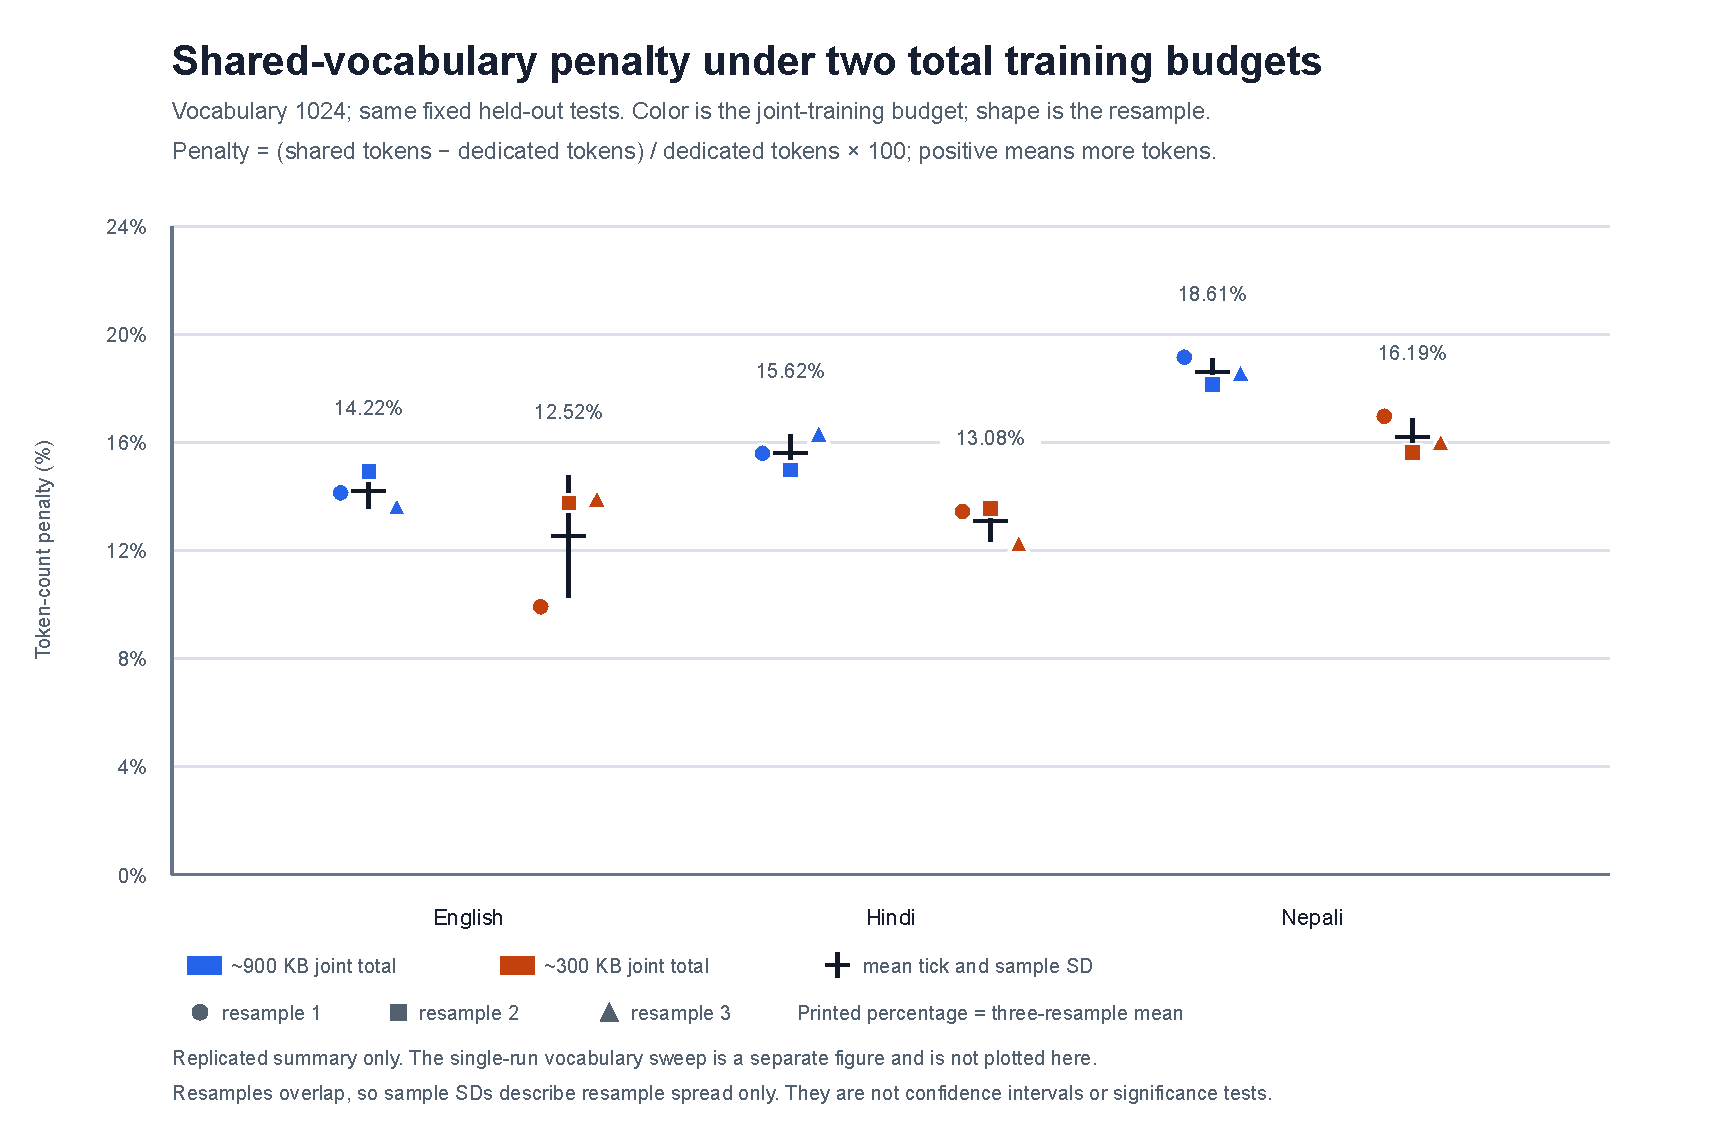
\includegraphics[width=0.98\textwidth]
{figures/budget_comparison.pdf}
\caption{Shared-vocabulary penalty at vocabulary 1,024
under the two replicated budgets. Points are the three
saved resamples. The number is their mean, and the bar
is the sample standard deviation. Overlapping resamples
make the standard deviations descriptive.}
\label{fig:budgets}
\end{figure*}

\subsection{Percentage penalties and absolute token counts}

The matched-budget means are lower than the
fixed-per-language means by about 1.69, 2.54, and
2.42 percentage points.

The arithmetic mean of the three token counts is higher
in the matched regime for every language and for both
the dedicated and joint condition.

Dedicated English token counts rise from a three-replicate
mean of 35,363.33 to 36,851.67, while joint counts rise
from 40,390.33 to 41,462.33.

Hindi moves from 44,383.33 to 46,014.67 dedicated and
from 51,317.33 to 52,032.00 joint.

Nepali moves from 53,641.00 to 55,872.00 dedicated
and from 63,625.33 to 64,919.67 joint.

The dedicated denominator grows by more, in relative
terms, than the joint numerator, so the ratio falls
while both encodings lengthen.

\begin{center}
\footnotesize
\setlength{\tabcolsep}{3pt}
\begin{tabular}{@{}lrrrr@{}}
\toprule
 & \multicolumn{2}{c}{About 300k bytes each}
 & \multicolumn{2}{c}{Matched subsets} \\
\cmidrule(lr){2-3}\cmidrule(lr){4-5}
Language & Dedicated & Joint & Dedicated & Joint \\
\midrule
English & 35,363.33 & 40,390.33 & 36,851.67 & 41,462.33 \\
Hindi & 44,383.33 & 51,317.33 & 46,014.67 & 52,032.00 \\
Nepali & 53,641.00 & 63,625.33 & 55,872.00 & 64,919.67 \\
\bottomrule
\end{tabular}

\captionof{table}{Mean held-out token counts across the
three replicates.}
\label{tab:absolute}
\end{center}

\subsection{Counterfactual vocabulary augmentation}

The augmentation analysis asks whether dedicated-tokenizer
pieces missing from the shared vocabulary can reduce
the token-count penalty.

The baseline Nepali Devanagari-specific penalty is
25.23\%. As eligible Nepali pieces are appended to copies
of the shared tokenizer, this penalty decreases.

Table~\ref{tab:augmentation} reports the mean values
provided by the augmentation experiment.

\begin{center}
\small
\begin{tabular}{@{}rr@{}}
\toprule
Nepali pieces added & Devanagari penalty (\%) \\
\midrule
0 & 25.23 \\
25 & 22.72 \\
50 & 20.44 \\
100 & 16.66 \\
200 & 10.48 \\
All eligible ($\sim$340) & 3.63 \\
\bottomrule
\end{tabular}

\captionof{table}{Nepali Devanagari-specific token-count
penalty under counterfactual vocabulary augmentation.}
\label{tab:augmentation}
\end{center}

At 100 added pieces, the Devanagari penalty decreases
from 25.23\% to 16.66\%. With all eligible pieces,
approximately 340, the penalty falls to 3.63\%.

The overall Nepali token-count penalty also decreases:
from 18.61\% at baseline to 11.77\% at 100 pieces,
6.91\% at 200 pieces, and 1.55\% with all eligible pieces.

These findings indicate that the missing dedicated
vocabulary pieces can account for a substantial portion
of the measured penalty under this augmentation procedure.

The effect is not restricted to Nepali. Adding Nepali
pieces also changes Hindi token counts because some
byte strings can be used across both languages.
However, the largest reductions occur in the language
whose dedicated pieces are being restored.

The Hindi-specific augmentation control similarly
reduces the Hindi Devanagari penalty. Adding 100
eligible Hindi pieces reduces it from 16.28\% to 9.43\%.

The random-order control shows that frequency-ranked
additions perform better than random additions at
smaller budgets in the reported comparisons. At the
full eligible budget, both procedures use the same
candidate pool.

The combined Hindi--Nepali condition also reduces
the Nepali penalty. Its Devanagari penalty reaches
14.96\% at 100 additions per language and 6.97\%
at 200 additions per language.

These combined results should be interpreted separately
from the Nepali-only condition because the combined
procedure uses additions from both languages.

\subsection{Word fragmentation and boundary analysis}

The augmentation analysis also evaluates how often
Nepali words are fragmented into more shared-tokenizer
pieces than dedicated-tokenizer pieces.

At baseline, 46.6\% of word occurrences have more
shared tokens, with a mean increase of 0.530 tokens
per word occurrence.

After adding 100 Nepali pieces, the proportion decreases
to 34.1\%, and the mean additional tokens per word
decreases to 0.328.

At 200 additions, 24.3\% of word occurrences have
more shared tokens, with a mean increase of 0.185.

With all eligible additions, the proportion decreases
to 14.2\%, and the mean additional tokens per word
decreases to 0.026.

The median increase remains zero, indicating that
the difference is concentrated in a subset of word
occurrences rather than being uniform across all words.

Boundary decomposition provides a complementary view.
The net extra token count decreases from 9,984 at
baseline to 6,314 at 100 additions and 829 with all
eligible additions.

The number of extra cuts inside strings absent from
the shared vocabulary decreases from 13,537 at baseline
to 8,935 at 100 additions and 3,063 with all eligible
additions.

These counts indicate that vocabulary augmentation
reduces both the frequency of word-level fragmentation
and the number of additional token boundaries associated
with missing dedicated pieces.

% --------------------------------------------------
% 7. Discussion
% --------------------------------------------------

\section{Discussion}

The original experiments show that the joint 1,024-token
vocabulary uses more held-out tokens than the dedicated
vocabulary in all nine comparisons under the fixed
per-language training regime.

The same is true when both conditions use the same
100,000-byte subsets.

In the one balanced selection, the penalty is positive
at 512, 1,024, and 2,048 for all three languages.

Those statements are limited to this corpus, this trainer,
these budgets, and this metric.

\subsection{Interpreting the training-data comparison}

The budget comparison supports a narrower conclusion
than a causal claim about data volume.

Moving from the first regime to the second changes
the dedicated sample, the joint sample, and which
documents appear.

The joint model sees less text, and the dedicated model
sees less text as well.

The percentage gap narrows while both token counts grow.
A design that held the dedicated data fixed and changed
only the joint budget was not run.

Shared Devanagari orthography did not remove the penalty
for Hindi and Nepali.

Nepali has the largest mean penalty in both replicated
regimes. This sample cannot separate script, morphology,
web-register mix, and the small document counts.

\subsection{Can language-specific pieces recover the penalty?}

The counterfactual augmentation analysis provides
additional evidence about the relationship between
language-specific vocabulary coverage and held-out
tokenization efficiency.

For Nepali, adding dedicated-tokenizer pieces that are
absent from the original shared vocabulary reduces the
Devanagari-specific penalty substantially.

The reduction is progressive across the tested budgets.
At 100 added pieces, the penalty decreases from 25.23\%
to 16.66\%. At 200 pieces, it reaches 10.48\%.
With all eligible pieces, it reaches 3.63\%.

The overall Nepali penalty follows a similar pattern,
decreasing from 18.61\% to 1.55\% with all eligible
pieces.

The word-fragmentation analysis supports this interpretation.
The proportion of word occurrences with more shared
tokens decreases from 46.6\% to 14.2\%.

Together, these results suggest that missing
language-specific vocabulary pieces account for a
substantial portion of the measured Nepali tokenization
penalty under this particular intervention.

However, this experiment does not demonstrate that
a newly trained shared tokenizer would learn the same
pieces or achieve the same reduction.

The augmentation procedure preserves the original merge
order and appends new merges after existing ones.
Consequently, original merges retain priority over
the appended merges.

The resulting tokenizer is not equivalent to a tokenizer
trained from scratch with the augmented vocabulary.

The experiment therefore demonstrates a conditional
recovery under vocabulary addition, not a fixed-capacity
solution to multilingual vocabulary allocation.

\subsection{Implications for vocabulary sharing}

The original comparison and the augmentation analysis
provide complementary evidence.

The first establishes that the shared vocabulary uses
more held-out tokens in the tested conditions.

The second indicates that restoring eligible
language-specific pieces can reduce a substantial part
of this difference, especially for Nepali.

Neither result determines whether a shared vocabulary
is preferable for a downstream multilingual model.

A tokenizer that uses more tokens can still help or hurt
a downstream model. We did not train one.

The result sits beside, and does not replace, studies
that allocate vocabulary or measure task quality
\citep{chung-etal-2020-improving,liang-etal-2023-xlm,
brahma-etal-2026-multilingual,ali-etal-2024-tokenizer}.

% --------------------------------------------------
% 8. Limitations
% --------------------------------------------------

\section{Limitations}

The source stream is unpinned, so the processed files
cannot be assumed to reappear from the dataset name alone.

The audit does not establish provenance or the absence
of pre-split contamination.

Resamples overlap, and three is too small a set for
a significance claim even if they did not.

The sweep selector and the resample selector do not
implement the byte cap in exactly the same way, although
both saved files are reported with exact byte counts.

The matched control exists only at vocabulary 1,024.

At that size the shared condition uses one 1,024-entry
vocabulary, and the three dedicated tokenizers
collectively use 3,072 vocabulary entries.

The experiment matches vocabulary size per tokenizer,
not aggregate vocabulary capacity.

The results characterize that specific comparison.
They do not isolate the effect of sharing under an
equal aggregate vocabulary budget, because no such
condition was trained.

The counterfactual augmentation experiment has additional
limitations.

First, the augmented vocabularies grow beyond the
original 1,024-entry shared vocabulary. The experiment
therefore does not preserve a fixed vocabulary budget.

Second, the new merges are appended after the original
merge list. The original merge priorities are preserved,
and the augmented tokenizer is not retrained from
scratch.

Third, candidates whose child byte strings are not
already individual tokens in the original shared
vocabulary are excluded. The results therefore describe
only the eligible candidate subset.

Fourth, the experiment does not establish whether the
same vocabulary pieces would be learned under a
fixed-capacity training procedure.

The augmentation results are based on the reported
experiment outputs. An independent source-code-level
audit of the augmentation implementation remains
necessary before treating the implementation details
as fully validated.

Grapheme and akshara tokenization are outside the
main comparison.

No downstream, transfer, or morphological evaluation
was run.

The source dataset's license, takedown status, and
personal information in the saved lines were not
independently audited.

% --------------------------------------------------
% 9. Conclusion
% --------------------------------------------------

\section{Conclusion}

On this English, Hindi, and Nepali sample, a fully
shared byte-level BPE vocabulary of 1,024 tokens
encodes held-out text with more tokens than a dedicated
vocabulary of the same requested size.

The penalty appears in every saved resample when
each language supplies about 300,000 training bytes,
and it remains when dedicated and joint training use
the same subsets of about 100,000 bytes.

The second setting has a smaller percentage penalty
and a larger absolute token count for both models.

The counterfactual augmentation analysis shows that
adding eligible dedicated-tokenizer pieces can
substantially reduce the measured tokenization penalty,
particularly for Nepali.

The Nepali Devanagari-specific penalty decreases
from 25.23\% at baseline to 16.66\% with 100 added
pieces and 3.63\% with all eligible pieces.

The corresponding overall Nepali penalty decreases
from 18.61\% to 1.55\%.

These results indicate that missing language-specific
pieces account for a substantial portion of the observed
penalty under the append-only augmentation procedure.

They do not establish that a retrained tokenizer with
the original fixed vocabulary budget would achieve
the same result.

Taken together, the experiments provide an intrinsic
token-count comparison and a counterfactual vocabulary
analysis for this English--Hindi--Nepali corpus,
this byte-level BPE implementation, and these
training conditions.

They are not a general law of multilingual tokenization,
and they are not evidence about downstream model quality.

% --------------------------------------------------
% Ethics and data
% --------------------------------------------------

\section*{Ethics and data}

The text is web data distributed through the named
Hugging Face dataset.

The dataset card states a CC0 license and points to
HPLT~3.0 as an upstream source.

This study did not independently audit the license,
take-down status, or personal information in the
saved lines.

The experimental subset is small and is used only
to count tokenizer output.

The code, manifests, model files, and result JSON
needed to recompute the original tables are in the
project directory.

% --------------------------------------------------
% References
% --------------------------------------------------

\FloatBarrier
\balance
\bibliography{references}

\end{document}
